
%(BEGIN_QUESTION)
% Copyright 2006, Tony R. Kuphaldt, released under the Creative Commons Attribution License (v 1.0)
% This means you may do almost anything with this work of mine, so long as you give me proper credit

Use Bernoulli's equation to calculate the pressure at the throat of this ``venturi'' tube, assuming water flowing at a rate of 15 cubic feet per second (15 ft$^{3}$/s), with a weight density ($\gamma$) of 62.4 lb/ft$^{3}$ and a mass density ($\rho$) of 1.951 slugs/ft$^{3}$:

$$\includegraphics[width=15.5cm]{i00451x01.eps}$$

Two versions of Bernoulli's equation are shown here, complete with descriptions of the variables and all the proper units of measurement.  Either one should yield the same result:

\vskip 10pt

$$z_1 \rho g + {v_1^2 \rho \over 2} + P_1 = z_2 \rho g + {v_2^2 \rho \over 2} + P_2$$

\vskip 10pt

$$z_1 + {v_1^2 \over {2 g}} + {P_1 \over \gamma} = z_2 + {v_2^2 \over {2 g}} + {P_2 \over \gamma}$$

\vskip 10pt

\noindent
Where,

$z$ = Height of fluid, in feet (ft)

$\rho$ = Mass density of fluid, in slugs per cubic foot (slug/ft$^{3}$)

$\gamma$ = Weight density of fluid ($\gamma = \rho g$), in pounds per cubic foot (lb/ft$^{3}$)

$g$ = Acceleration of gravity (32.2 ft/s$^{2}$)

$v$ = Velocity of fluid, in feet per second (ft/s)

$P$ = Pressure of fluid, in pounds per square foot (lb/ft$^{2}$)

\vskip 10pt

Lastly, calculate the {\it differential pressure} (DP) generated by this venturi tube.

\vskip 10pt

\vskip 20pt \vbox{\hrule \hbox{\strut \vrule{} {\bf Suggestions for Socratic discussion} \vrule} \hrule}

\begin{itemize}
\item{} The textbook outlines a general strategy for generating a problem-solving plan when tackling problems with complex mathematical formulae.  Specifically, this strategy involved writing out the formulae and linking variables between formulae with arrow symbols.  Explain how this strategy works, and show how it may be applied to the solution of this problem.
\item{} A very helpful strategy for tackling Bernoulli's equation problems is to create a table in which to place each of the ``head'' terms of that equation.  Explain why this is helpful to manage this specific type of problem.
\item{} Venturi tubes are often used to create {\it vacuums}, by passing some fluid through the venturi at high speed and then providing a vacuum tap at the throat.  Automobile engine carburetors and atomizing spray guns are two prominent examples of this.  In industry, another example is the so-called {\it steam eductor}, using a jet of high-velocity steam through a venturi to create continuous suction (vacuum).  Are there any advantages to using eductors to create vacuums as opposed to using mechanical vacuum pumps?  Are there any disadvantages to the use of eductors for creating vacuums?
\end{itemize}

\underbar{file i00451}
%(END_QUESTION)





%(BEGIN_ANSWER)

$P_2$ = 0.490 PSI (using top equation, with $\rho$ = 1.951 slugs/ft$^{3}$)

\vskip 10pt

$P_2$ = 0.531 PSI (using bottom equation, with $\gamma$ = 62.4 lb/ft$^{3}$)

\vskip 10pt

Hint: $v_1$ = $v_3$ = 19.1 ft/s ; $v_2$ = 110.0 ft/s ; $P_1$ = 11,520 lb/ft$^{2}$

\vskip 10pt

Note: even slight amounts of rounding error may add up to skew the $P_2$ pressure calculation so that it ends up being as high as 1 PSI instead of half of a PSI.  In order to avoid incurring rounding errors, you must store all intermediate calculated results in your calculator's memory locations rather than write them on paper and re-enter them.  This is a good practice in general, not only because it avoids unnecessary rounding being introduced into your calculations, but also because it completely avoids simple keystroke errors!

%(END_ANSWER)





%(BEGIN_NOTES)

% No blank lines allowed between lines of an \halign structure!
% I use comments (%) instead, so Tex doesn't choke.

$$\vbox{\offinterlineskip
\halign{\strut
\vrule \quad\hfil # \ \hfil & 
\vrule \quad\hfil # \ \hfil & 
\vrule \quad\hfil # \ \hfil \vrule \cr
\noalign{\hrule}
%
% First row
{\bf Head} & {\bf Calculation} at 12 inch tube & {\bf Value} \cr
%
\noalign{\hrule}
%
% Another row
$z_1 \rho g$ & (0 ft) (1.951 slugs/ft$^{3}$) (32.2 ft/s$^{2}$) & 0 lb/ft$^{2}$ \cr
%
\noalign{\hrule}
%
% Another row
$v_1^2 \rho / 2$ & (19.098 ft/s)$^{2}$ (1.951 slugs/ft$^{3}$) / 2 & 355.820 lb/ft$^{2}$ \cr
%
\noalign{\hrule}
%
% Another row
$P_1$ & (80 lb/in$^{2}$) (144 in$^{2}$/1 ft$^{2}$) & 11520 lb/ft$^{2}$ \cr
%
\noalign{\hrule}
%
% Another row
{\bf Total} &  0 lb/ft$^{2}$ + 355.820 lb/ft$^{2}$ + 11520 lb/ft$^{2}$ & {\bf 11875.820 lb/ft$^{2}$} \cr
%
\noalign{\hrule}
} % End of \halign 
}$$ % End of \vbox

\vskip 10pt

% No blank lines allowed between lines of an \halign structure!
% I use comments (%) instead, so Tex doesn't choke.

$$\vbox{\offinterlineskip
\halign{\strut
\vrule \quad\hfil # \ \hfil & 
\vrule \quad\hfil # \ \hfil & 
\vrule \quad\hfil # \ \hfil \vrule \cr
\noalign{\hrule}
%
% First row
{\bf Head} & {\bf Calculation} at 5 inch tube & {\bf Value} \cr
%
\noalign{\hrule}
%
% Another row
$z_2 \rho g$ & (0 ft) (1.951 slugs/ft$^{3}$) (32.2 ft/s$^{2}$) & 0 lb/ft$^{2}$ \cr
%
\noalign{\hrule}
%
% Another row
$v_2^2 \rho / 2$ & (110.01 ft/s)$^{2}$ (1.951 slugs/ft$^{3}$) / 2 & 11805.245 lb/ft$^{2}$ \cr
%
\noalign{\hrule}
%
% Another row
$P_2$ & (?? lb/in$^{2}$) (144 in$^{2}$/1 ft$^{2}$) & ??? lb/ft$^{2}$ \cr
%
\noalign{\hrule}
%
% Another row
{\bf Total} &  0 lb/ft$^{2}$ + 11805.245 lb/ft$^{2}$ + ??? lb/ft$^{2}$ & {\bf 11875.820 lb/ft$^{2}$} \cr
%
\noalign{\hrule}
} % End of \halign 
}$$ % End of \vbox

$$P_2 = 11875.820 \hbox{ lb/ft}^2 - 11805.245 \hbox{ lb/ft}^2 = 70.575 \hbox{ lb/ft}^2 = 0.4901 \hbox{ PSI}$$

\vskip 10pt

If the second version of Bernoulli's equation is used, you get a slightly different result for $P_2$ of 0.531 PSI instead of 0.490 PSI.  The difference between the two answers lies in the imperfect equivalence of 1.951 slugs/ft$^{3}$ (mass density) and 62.4 lb/ft$^{3}$ (weight density) for water.

\vskip 10pt

$\Delta P$ = $P_1 - P_2$ = 80 PSI $-$ 0.4901 PSI = 79.510 PSI

%INDEX% Physics, dynamic fluids: Bernoulli's equation

%(END_NOTES)


